
%*******************************************************************************
%***********************************    Background   *****************************
%*******************************************************************************
%!TEX root = 0.main.tex

\setcounter{page}{1}



%********************************** %First Section  **************************************
\section {Introduction and general background} 

\subsection{Introduction}

Neural Networks (NNs) are popular algorithms for regression and classification tasks. Taking as example classification tasks of mapping the image $I$ into its correct label $C_I$, neural networks perform multiple combinations of linear and non-linear transformations of the image $I$ to assign it a label in $\mathcal C$.  The first \textit{layer} of a neural network transforms the input image $I$ in a vector $\mathbf f_1$ through a function $\phi_1$. $\mathbf f_1$ is used as input of the following layer that transforms it in a second vector $\mathbf f_2$ through a second function $\phi_2$, and so on, until the original image $I$ is mapped into a label $C_I$ by the last, $n$-th layer of the neural network:
$$C_I = \phi_n \circ \phi_{n-1}\circ ... \phi_2\circ\phi_1 (I)$$
 Given a large \textit{training set} of labeled images, a neural network is capable of learning the optimal transformations $\phi_i$ that let it map the input image to its correct label. Since the functions $\phi_i$ have many degrees of freedom - even millions - a neural network is able to learn very complex transformations. This characteristic makes NNs the optimal tool for complex tasks such as image classification, image segmentation, speech recognition and natural language processing.\\

Convolutional Neural Networks (CNNs) are a specific class of neural networks whose layer structure has been specifically designed for image recognition and segmentation. For this purpose, they don't have all the degrees of freedom of a normal, \textit{fully connected} neural network described above: each layer of a CNN has been constrained to only learn transformations of the input that are \textit{invariant} to translation of the input. This means that if used in an image classification task, a translation of the input image will not result in a change of class. The function $\phi_i$ of a CNN are \textit{convolutions} with some kernel that was learned during the training phase. Thanks to their design, training of CNNs is faster - thanks to the smaller number of parameters to be learned compared to a fully connected NN -, it is easier -since there's no need of artificially \textit{augmenting} the dataset with translated copies of the same image -, and leads to very accurate results.\\

Spherical convolutional neural networks (SCNNs) are NNs that have been specifically designed to deal with spherical data, whose layer design makes them \textit{equivariant to rotations of the input}.  Examples of tasks where data is naturally represented on a sphere are (i) climate science, where data is sampled on the surface of the Earth, (ii) cosmology, where observations are naturally projected on a sphere centered around the observer (see Figure \ref{fig:cosmicradiation}), and (iii) virtual reality, where the images are represented on a sphere centered around the player. Being able to come up with designs that are equivariant to rotations brings with it all the advantages that traditional CNNs have brought for traditional (euclidean) image classification tasks: training is faster, easier and results are very accurate. The transformations $\phi_i$ that each layer of a SCNN performs is a \textit{spherical convolution} of the input vector with a kernel learned during the training phase. 

\begin{figure}
	\centering
	\caption{\label{fig:cosmicradiation} Cosmic microwave background map, the oldest electromagnetic radiation in the universe. Source: Wikipedia}
	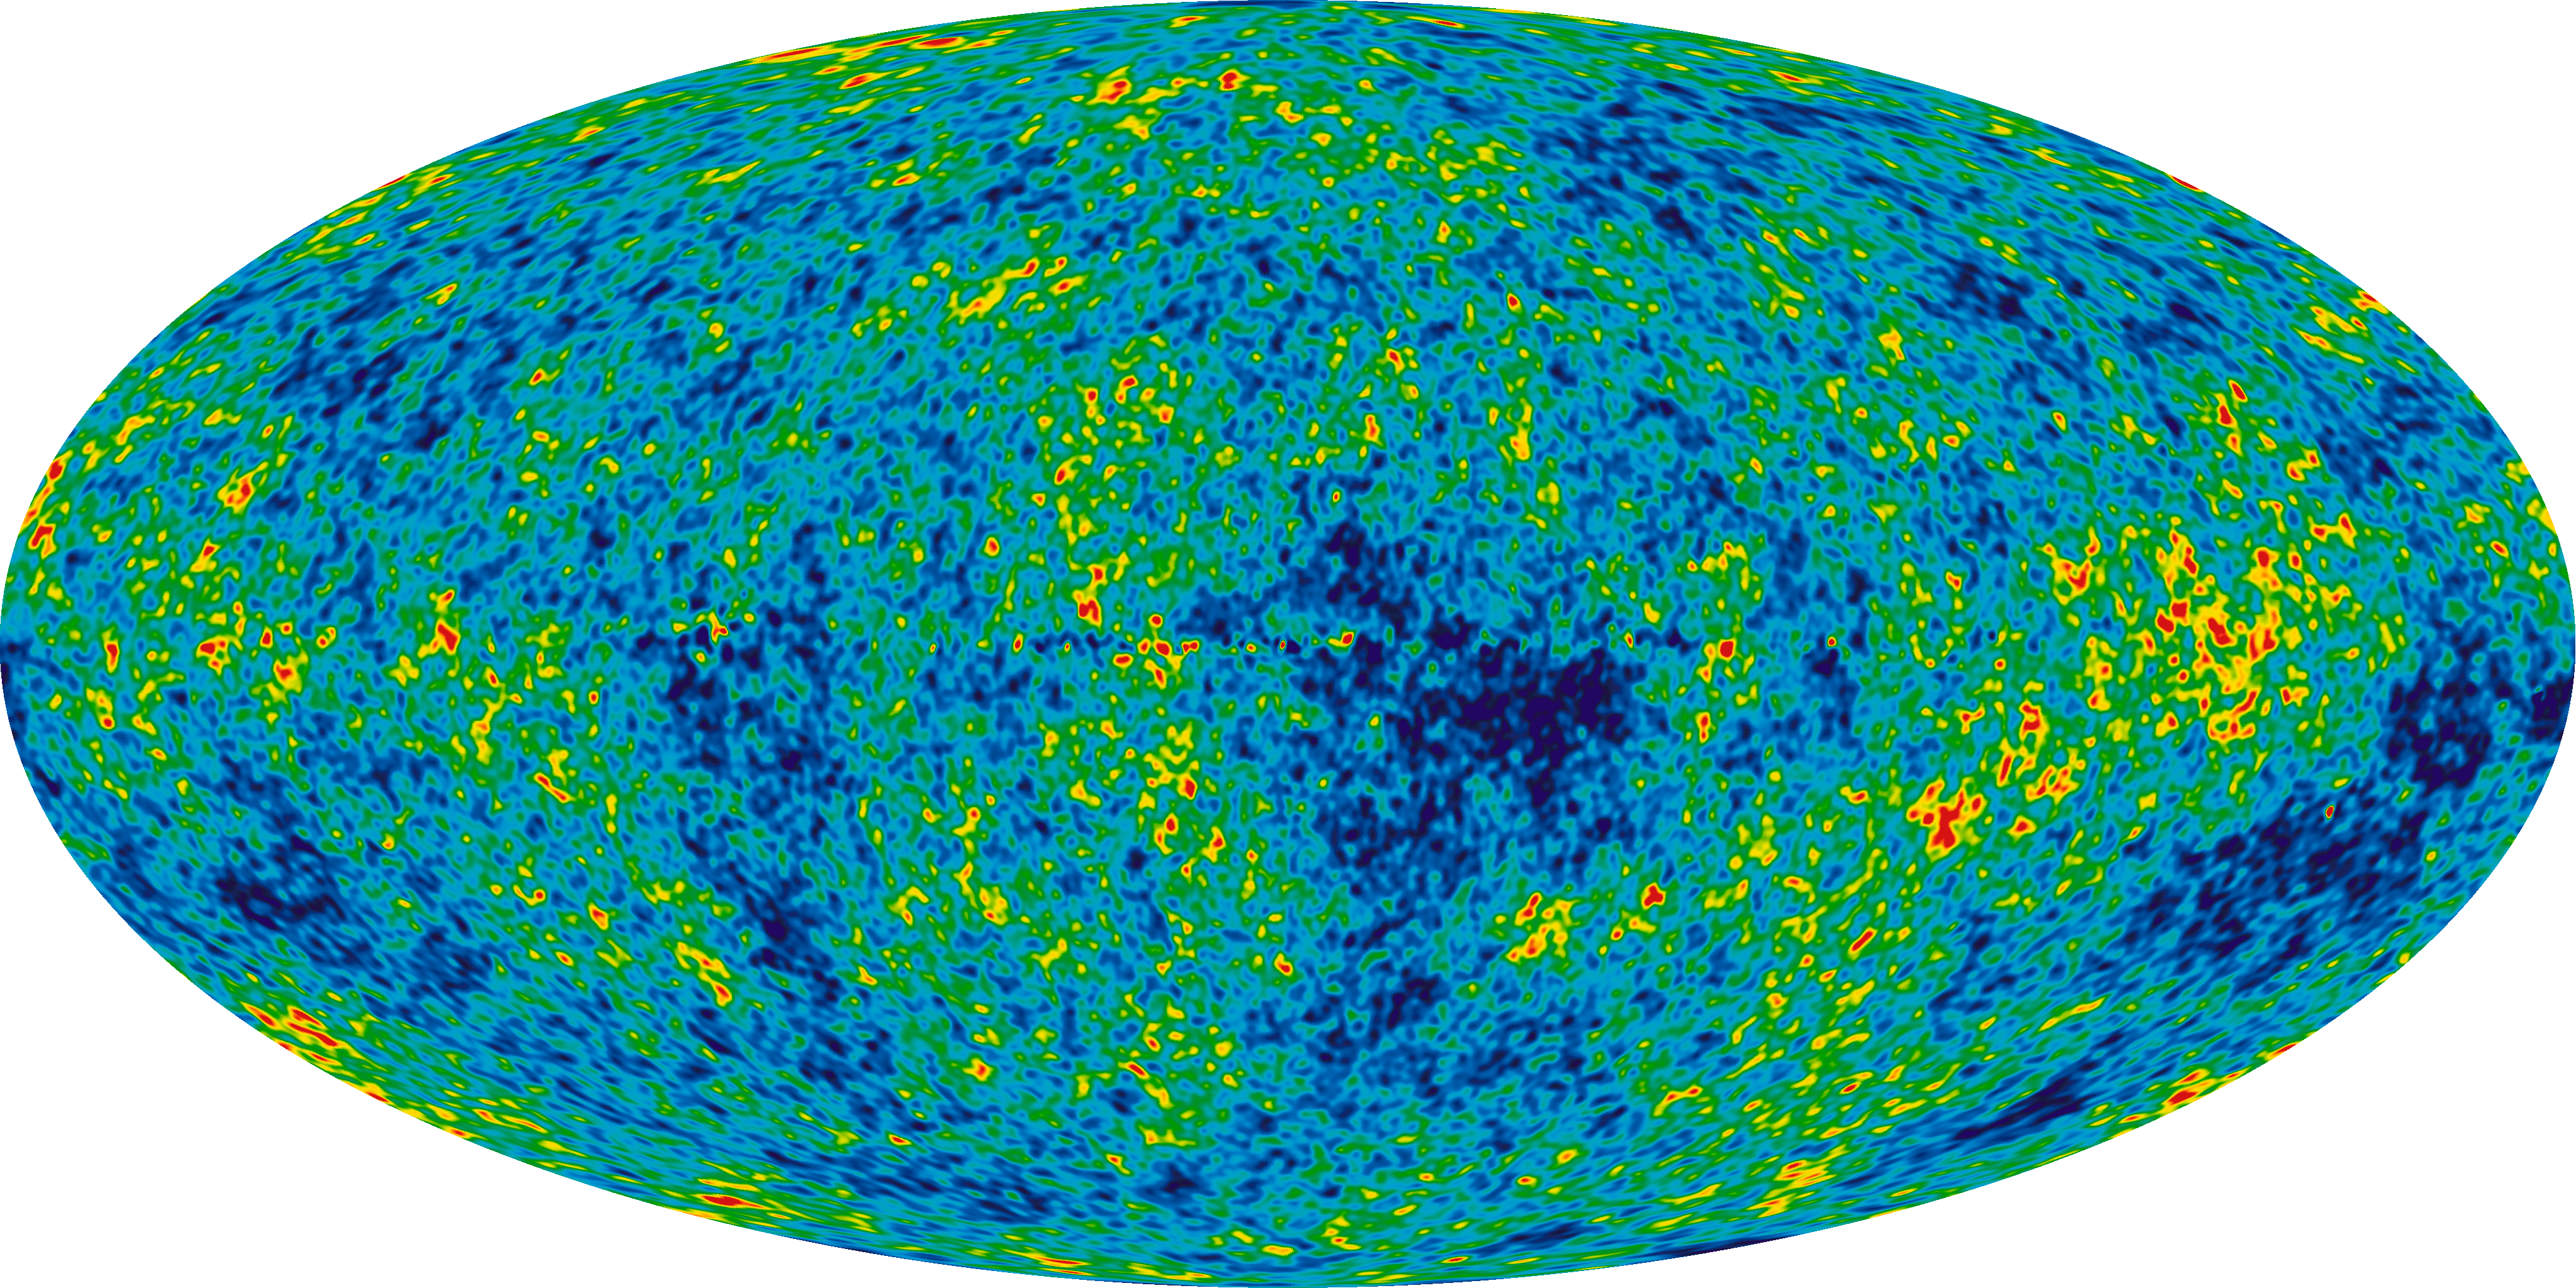
\includegraphics[width=0.4\textwidth]{figs/literaturereview/WMAP.png}
\end{figure}
One of the main issues with traditional SCNNs is the computational complexity of computing at each layer the Spherical Harmonic Transform (SHT) of the data to perform the convolution in the spectral domain. Perraudin et al. \cite{DeepSphere} proposed a Graph Convolutional Neural Network (GCNN) that is almost equivariant to rotations, replacing the SHT with a more efficient Graph Convolution.

In Chapter 1 we start by presenting fundamental concepts of spectral theory on the sphere and we present classical ways of building rotation equivariant neural networks through the use of the SHT.  We present then some basics of Graph Spectral Theory useful to introduce the work of Perraudin et al. DeepSphere \cite{DeepSphere}. We present then a well suited way to build a graph to approximate the Laplace-Beltrami operator on a manifold, the Heat Kernel Graph Laplacian (HKGL) together with some convergence results. In Chapter 2 we study the spectral properties of the graph Laplacian matrix $\mathbf L$ used by Perraudin et al. and we show a way to build a graph $G'$ such that the corresponding graph Laplacian matrix $\mathbf L'$ shows better spectral properties. In Chapter 3 we investigate other different methods of building the matrix $\mathbf L$ better suited to non uniform sampling measures. In particular, we study the Finite Element Method approximation of the Laplace-Beltrami operator on the sphere. We compare the FEM and the graph Laplacian on different samplings of the sphere. We finish by discussing the general problem of how to incorporate geometrical informations about the sphere in the graph, a purely topological object.

\subsection{Fourier Transforms and Convolutions on the 2-Sphere}
[Review of \textit{Computing Fourier Transforms and Convolutions on the 2-Sphere}]
\subsection{Spherical Convolutional Neural Networks}
[Review of \textit{Spherical CNNs}]
\subsection{Graph Spectral Theory} \label{sec:Chapter1: Spectral Graph Theory}
[Review of \textit{The emerging field of Graph Signal Processing}]
\subsection{Deep Sphere V1.0}
[Review of \textit{Deep Sphere}]
\subsection{Belkin's trinity}
[Review of \textit{the Belkin's trinity}]

\subsubsection{Towards a theoretical foundation of Laplacian-based manifold methods}

\subsubsection{Consistency of Spectral Clustering}

\subsubsection{Convergence of Laplacian Eigenmaps}
